% Options for packages loaded elsewhere
\PassOptionsToPackage{unicode}{hyperref}
\PassOptionsToPackage{hyphens}{url}
%
\documentclass[
  english,
  man]{apa6}
\usepackage{lmodern}
\usepackage{amssymb,amsmath}
\usepackage{ifxetex,ifluatex}
\ifnum 0\ifxetex 1\fi\ifluatex 1\fi=0 % if pdftex
  \usepackage[T1]{fontenc}
  \usepackage[utf8]{inputenc}
  \usepackage{textcomp} % provide euro and other symbols
\else % if luatex or xetex
  \usepackage{unicode-math}
  \defaultfontfeatures{Scale=MatchLowercase}
  \defaultfontfeatures[\rmfamily]{Ligatures=TeX,Scale=1}
\fi
% Use upquote if available, for straight quotes in verbatim environments
\IfFileExists{upquote.sty}{\usepackage{upquote}}{}
\IfFileExists{microtype.sty}{% use microtype if available
  \usepackage[]{microtype}
  \UseMicrotypeSet[protrusion]{basicmath} % disable protrusion for tt fonts
}{}
\makeatletter
\@ifundefined{KOMAClassName}{% if non-KOMA class
  \IfFileExists{parskip.sty}{%
    \usepackage{parskip}
  }{% else
    \setlength{\parindent}{0pt}
    \setlength{\parskip}{6pt plus 2pt minus 1pt}}
}{% if KOMA class
  \KOMAoptions{parskip=half}}
\makeatother
\usepackage{xcolor}
\IfFileExists{xurl.sty}{\usepackage{xurl}}{} % add URL line breaks if available
\IfFileExists{bookmark.sty}{\usepackage{bookmark}}{\usepackage{hyperref}}
\hypersetup{
  pdftitle={MSDS680 - Week 4 - Decision Trees},
  pdfauthor={Benjamin Siebold},
  pdflang={en-EN},
  pdfkeywords={keywords},
  hidelinks,
  pdfcreator={LaTeX via pandoc}}
\urlstyle{same} % disable monospaced font for URLs
\usepackage{color}
\usepackage{fancyvrb}
\newcommand{\VerbBar}{|}
\newcommand{\VERB}{\Verb[commandchars=\\\{\}]}
\DefineVerbatimEnvironment{Highlighting}{Verbatim}{commandchars=\\\{\}}
% Add ',fontsize=\small' for more characters per line
\usepackage{framed}
\definecolor{shadecolor}{RGB}{248,248,248}
\newenvironment{Shaded}{\begin{snugshade}}{\end{snugshade}}
\newcommand{\AlertTok}[1]{\textcolor[rgb]{0.94,0.16,0.16}{#1}}
\newcommand{\AnnotationTok}[1]{\textcolor[rgb]{0.56,0.35,0.01}{\textbf{\textit{#1}}}}
\newcommand{\AttributeTok}[1]{\textcolor[rgb]{0.77,0.63,0.00}{#1}}
\newcommand{\BaseNTok}[1]{\textcolor[rgb]{0.00,0.00,0.81}{#1}}
\newcommand{\BuiltInTok}[1]{#1}
\newcommand{\CharTok}[1]{\textcolor[rgb]{0.31,0.60,0.02}{#1}}
\newcommand{\CommentTok}[1]{\textcolor[rgb]{0.56,0.35,0.01}{\textit{#1}}}
\newcommand{\CommentVarTok}[1]{\textcolor[rgb]{0.56,0.35,0.01}{\textbf{\textit{#1}}}}
\newcommand{\ConstantTok}[1]{\textcolor[rgb]{0.00,0.00,0.00}{#1}}
\newcommand{\ControlFlowTok}[1]{\textcolor[rgb]{0.13,0.29,0.53}{\textbf{#1}}}
\newcommand{\DataTypeTok}[1]{\textcolor[rgb]{0.13,0.29,0.53}{#1}}
\newcommand{\DecValTok}[1]{\textcolor[rgb]{0.00,0.00,0.81}{#1}}
\newcommand{\DocumentationTok}[1]{\textcolor[rgb]{0.56,0.35,0.01}{\textbf{\textit{#1}}}}
\newcommand{\ErrorTok}[1]{\textcolor[rgb]{0.64,0.00,0.00}{\textbf{#1}}}
\newcommand{\ExtensionTok}[1]{#1}
\newcommand{\FloatTok}[1]{\textcolor[rgb]{0.00,0.00,0.81}{#1}}
\newcommand{\FunctionTok}[1]{\textcolor[rgb]{0.00,0.00,0.00}{#1}}
\newcommand{\ImportTok}[1]{#1}
\newcommand{\InformationTok}[1]{\textcolor[rgb]{0.56,0.35,0.01}{\textbf{\textit{#1}}}}
\newcommand{\KeywordTok}[1]{\textcolor[rgb]{0.13,0.29,0.53}{\textbf{#1}}}
\newcommand{\NormalTok}[1]{#1}
\newcommand{\OperatorTok}[1]{\textcolor[rgb]{0.81,0.36,0.00}{\textbf{#1}}}
\newcommand{\OtherTok}[1]{\textcolor[rgb]{0.56,0.35,0.01}{#1}}
\newcommand{\PreprocessorTok}[1]{\textcolor[rgb]{0.56,0.35,0.01}{\textit{#1}}}
\newcommand{\RegionMarkerTok}[1]{#1}
\newcommand{\SpecialCharTok}[1]{\textcolor[rgb]{0.00,0.00,0.00}{#1}}
\newcommand{\SpecialStringTok}[1]{\textcolor[rgb]{0.31,0.60,0.02}{#1}}
\newcommand{\StringTok}[1]{\textcolor[rgb]{0.31,0.60,0.02}{#1}}
\newcommand{\VariableTok}[1]{\textcolor[rgb]{0.00,0.00,0.00}{#1}}
\newcommand{\VerbatimStringTok}[1]{\textcolor[rgb]{0.31,0.60,0.02}{#1}}
\newcommand{\WarningTok}[1]{\textcolor[rgb]{0.56,0.35,0.01}{\textbf{\textit{#1}}}}
\usepackage{graphicx,grffile}
\makeatletter
\def\maxwidth{\ifdim\Gin@nat@width>\linewidth\linewidth\else\Gin@nat@width\fi}
\def\maxheight{\ifdim\Gin@nat@height>\textheight\textheight\else\Gin@nat@height\fi}
\makeatother
% Scale images if necessary, so that they will not overflow the page
% margins by default, and it is still possible to overwrite the defaults
% using explicit options in \includegraphics[width, height, ...]{}
\setkeys{Gin}{width=\maxwidth,height=\maxheight,keepaspectratio}
% Set default figure placement to htbp
\makeatletter
\def\fps@figure{htbp}
\makeatother
\setlength{\emergencystretch}{3em} % prevent overfull lines
\providecommand{\tightlist}{%
  \setlength{\itemsep}{0pt}\setlength{\parskip}{0pt}}
\setcounter{secnumdepth}{-\maxdimen} % remove section numbering
% Make \paragraph and \subparagraph free-standing
\ifx\paragraph\undefined\else
  \let\oldparagraph\paragraph
  \renewcommand{\paragraph}[1]{\oldparagraph{#1}\mbox{}}
\fi
\ifx\subparagraph\undefined\else
  \let\oldsubparagraph\subparagraph
  \renewcommand{\subparagraph}[1]{\oldsubparagraph{#1}\mbox{}}
\fi
% Manuscript styling
\usepackage{upgreek}
\captionsetup{font=singlespacing,justification=justified}

% Table formatting
\usepackage{longtable}
\usepackage{lscape}
% \usepackage[counterclockwise]{rotating}   % Landscape page setup for large tables
\usepackage{multirow}		% Table styling
\usepackage{tabularx}		% Control Column width
\usepackage[flushleft]{threeparttable}	% Allows for three part tables with a specified notes section
\usepackage{threeparttablex}            % Lets threeparttable work with longtable

% Create new environments so endfloat can handle them
% \newenvironment{ltable}
%   {\begin{landscape}\begin{center}\begin{threeparttable}}
%   {\end{threeparttable}\end{center}\end{landscape}}
\newenvironment{lltable}{\begin{landscape}\begin{center}\begin{ThreePartTable}}{\end{ThreePartTable}\end{center}\end{landscape}}

% Enables adjusting longtable caption width to table width
% Solution found at http://golatex.de/longtable-mit-caption-so-breit-wie-die-tabelle-t15767.html
\makeatletter
\newcommand\LastLTentrywidth{1em}
\newlength\longtablewidth
\setlength{\longtablewidth}{1in}
\newcommand{\getlongtablewidth}{\begingroup \ifcsname LT@\roman{LT@tables}\endcsname \global\longtablewidth=0pt \renewcommand{\LT@entry}[2]{\global\advance\longtablewidth by ##2\relax\gdef\LastLTentrywidth{##2}}\@nameuse{LT@\roman{LT@tables}} \fi \endgroup}

% \setlength{\parindent}{0.5in}
% \setlength{\parskip}{0pt plus 0pt minus 0pt}

% \usepackage{etoolbox}
\makeatletter
\patchcmd{\HyOrg@maketitle}
  {\section{\normalfont\normalsize\abstractname}}
  {\section*{\normalfont\normalsize\abstractname}}
  {}{\typeout{Failed to patch abstract.}}
\patchcmd{\HyOrg@maketitle}
  {\section{\protect\normalfont{\@title}}}
  {\section*{\protect\normalfont{\@title}}}
  {}{\typeout{Failed to patch title.}}
\makeatother
\shorttitle{Decision Trees and }
\keywords{keywords\newline\indent Word count: X}
\DeclareDelayedFloatFlavor{ThreePartTable}{table}
\DeclareDelayedFloatFlavor{lltable}{table}
\DeclareDelayedFloatFlavor*{longtable}{table}
\makeatletter
\renewcommand{\efloat@iwrite}[1]{\immediate\expandafter\protected@write\csname efloat@post#1\endcsname{}}
\makeatother
\usepackage{csquotes}
\ifxetex
  % Load polyglossia as late as possible: uses bidi with RTL langages (e.g. Hebrew, Arabic)
  \usepackage{polyglossia}
  \setmainlanguage[]{english}
\else
  \usepackage[shorthands=off,main=english]{babel}
\fi

\title{MSDS680 - Week 4 - Decision Trees}
\author{Benjamin Siebold\textsuperscript{}}
\date{}


\affiliation{\vspace{0.5cm}\textsuperscript{} Regis University}

\begin{document}
\maketitle

\hypertarget{introduction}{%
\section{Introduction}\label{introduction}}

\hypertarget{methodology}{%
\section{Methodology}\label{methodology}}

\hypertarget{set-up}{%
\subsection{Set Up}\label{set-up}}

\begin{Shaded}
\begin{Highlighting}[]
\KeywordTok{library}\NormalTok{(DataExplorer) }\CommentTok{#data exploration}
\KeywordTok{library}\NormalTok{(factoextra) }\CommentTok{#building wss and silhouette plots}
\KeywordTok{library}\NormalTok{(tidyverse) }\CommentTok{#data cleaning}
\KeywordTok{library}\NormalTok{(cluster) }\CommentTok{#applies HCA}
\KeywordTok{library}\NormalTok{(dendextend) }\CommentTok{#compares dendrograms}
\KeywordTok{library}\NormalTok{(caret) }\CommentTok{#dummy variables}

\KeywordTok{set.seed}\NormalTok{(}\DecValTok{422}\NormalTok{)}
\NormalTok{customers <-}\StringTok{ }\KeywordTok{read.csv}\NormalTok{(}\StringTok{'../Week-6/Wholesale customers data.csv'}\NormalTok{)}
\end{Highlighting}
\end{Shaded}

\hypertarget{data-clean}{%
\subsection{Data Clean}\label{data-clean}}

\begin{Shaded}
\begin{Highlighting}[]
\KeywordTok{summary}\NormalTok{(customers)}
\end{Highlighting}
\end{Shaded}

\begin{verbatim}
## Channel Region Fresh Milk
## Min.  :1.000 Min.  :1.000 Min.  : 3 Min.  : 55
## 1st Qu.:1.000 1st Qu.:2.000 1st Qu.: 3128 1st Qu.: 1533
## Median :1.000 Median :3.000 Median : 8504 Median : 3627
## Mean :1.323 Mean :2.543 Mean : 12000 Mean : 5796
## 3rd Qu.:2.000 3rd Qu.:3.000 3rd Qu.: 16934 3rd Qu.: 7190
## Max.  :2.000 Max.  :3.000 Max.  :112151 Max.  :73498
## Grocery Frozen Detergents_Paper Delicassen
## Min.  : 3 Min.  : 25.0 Min.  : 3.0 Min.  : 3.0
## 1st Qu.: 2153 1st Qu.: 742.2 1st Qu.: 256.8 1st Qu.:
408.2
## Median : 4756 Median : 1526.0 Median : 816.5 Median :
965.5
## Mean : 7951 Mean : 3071.9 Mean : 2881.5 Mean : 1524.9
## 3rd Qu.:10656 3rd Qu.: 3554.2 3rd Qu.: 3922.0 3rd Qu.:
1820.2
## Max.  :92780 Max.  :60869.0 Max.  :40827.0 Max.
:47943.0
\end{verbatim}

\begin{Shaded}
\begin{Highlighting}[]
\KeywordTok{str}\NormalTok{(customers)}
\end{Highlighting}
\end{Shaded}

\begin{verbatim}
## 'data.frame': 440 obs. of 8 variables:
## $ Channel : int 2 2 2 1 2 2 2 2 1 2 ...
## $ Region : int 3 3 3 3 3 3 3 3 3 3 ...
## $ Fresh : int 12669 7057 6353 13265 22615 9413 12126
7579 5963 6006 ...
## $ Milk : int 9656 9810 8808 1196 5410 8259 3199 4956
3648 11093 ...
## $ Grocery : int 7561 9568 7684 4221 7198 5126 6975 9426
6192 18881 ...
## $ Frozen : int 214 1762 2405 6404 3915 666 480 1669 425
1159 ...
## $ Detergents_Paper: int 2674 3293 3516 507 1777 1795
3140 3321 1716 7425 ...
## $ Delicassen : int 1338 1776 7844 1788 5185 1451 545
2566 750 2098 ...
\end{verbatim}

\begin{Shaded}
\begin{Highlighting}[]
\KeywordTok{plot_histogram}\NormalTok{(customers)}
\end{Highlighting}
\end{Shaded}

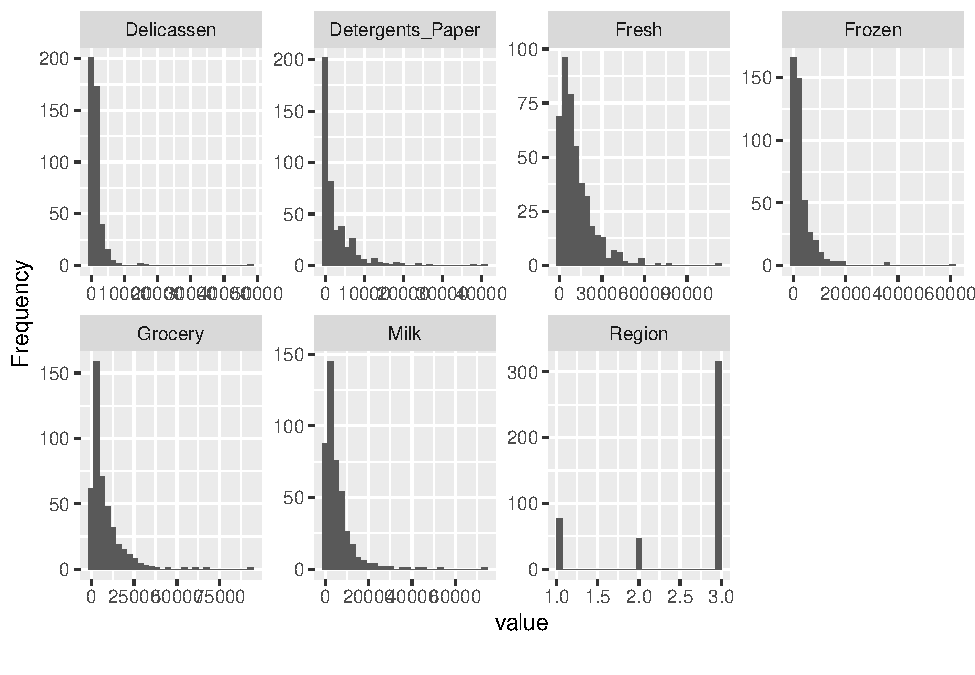
\includegraphics{MSDS680-Week-6-Kmeans-and-HCA_files/figure-latex/data clean-1.pdf}

\begin{Shaded}
\begin{Highlighting}[]
\NormalTok{customers_factor <-}\StringTok{ }\KeywordTok{as.data.frame}\NormalTok{(}\KeywordTok{lapply}\NormalTok{(customers[,}\KeywordTok{c}\NormalTok{(}\DecValTok{1}\NormalTok{,}\DecValTok{2}\NormalTok{)], as.factor))}
\NormalTok{customers_scaled <-}\StringTok{ }\KeywordTok{as.data.frame}\NormalTok{(}\KeywordTok{lapply}\NormalTok{(customers[,}\KeywordTok{c}\NormalTok{(}\DecValTok{3}\OperatorTok{:}\DecValTok{8}\NormalTok{)], scale))}
\NormalTok{dummy_vars <-}\StringTok{ }\KeywordTok{dummyVars}\NormalTok{(}\StringTok{'~.'}\NormalTok{, }\DataTypeTok{data=}\NormalTok{customers_factor,}\DataTypeTok{fullRank=}\NormalTok{T)}
\NormalTok{dummy_customers <-}\StringTok{ }\KeywordTok{as.data.frame}\NormalTok{(}\KeywordTok{predict}\NormalTok{(dummy_vars, }\DataTypeTok{newdata=}\NormalTok{customers_factor))}

\CommentTok{#creates dummy dataset without scales}
\NormalTok{clean_customers <-}\StringTok{ }\KeywordTok{cbind}\NormalTok{(dummy_customers,customers[,}\KeywordTok{c}\NormalTok{(}\DecValTok{3}\OperatorTok{:}\DecValTok{8}\NormalTok{)]) }
\CommentTok{#creates scaled dataset with dummy variables}
\NormalTok{scaled_clean_cust <-}\StringTok{ }\KeywordTok{cbind}\NormalTok{(dummy_customers, customers_scaled) }
\end{Highlighting}
\end{Shaded}

\hypertarget{kmeans-cluster-decision}{%
\subsection{Kmeans Cluster Decision}\label{kmeans-cluster-decision}}

\begin{Shaded}
\begin{Highlighting}[]
\KeywordTok{fviz_nbclust}\NormalTok{(clean_customers, kmeans, }\DataTypeTok{method =} \StringTok{'wss'}\NormalTok{)}
\end{Highlighting}
\end{Shaded}

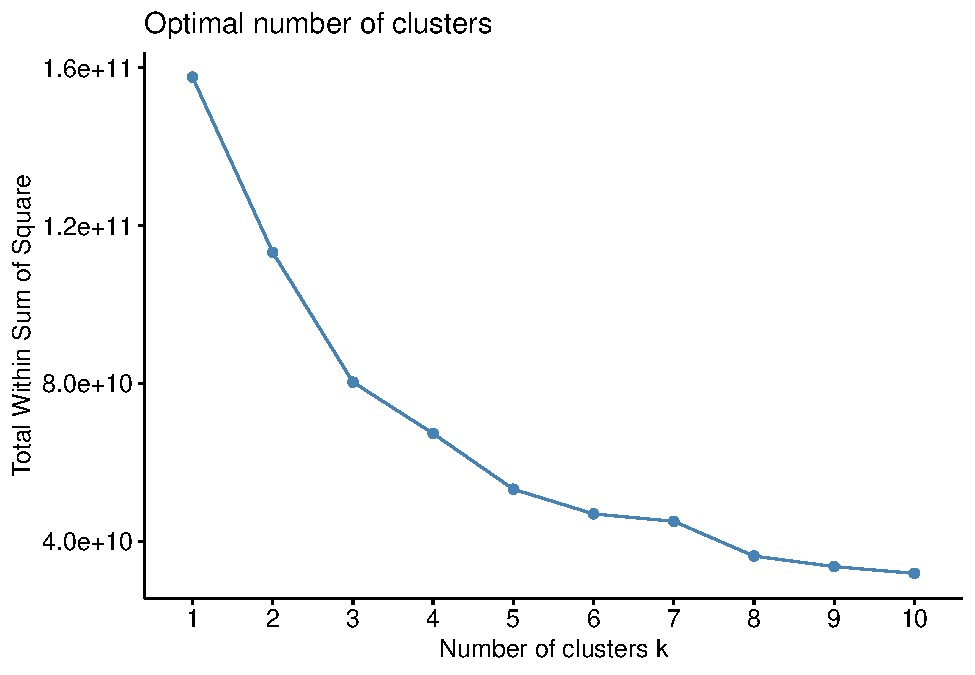
\includegraphics{MSDS680-Week-6-Kmeans-and-HCA_files/figure-latex/kmeans investigation-1.pdf}

\begin{Shaded}
\begin{Highlighting}[]
\KeywordTok{fviz_nbclust}\NormalTok{(scaled_clean_cust, kmeans, }\DataTypeTok{method =} \StringTok{'wss'}\NormalTok{)}
\end{Highlighting}
\end{Shaded}

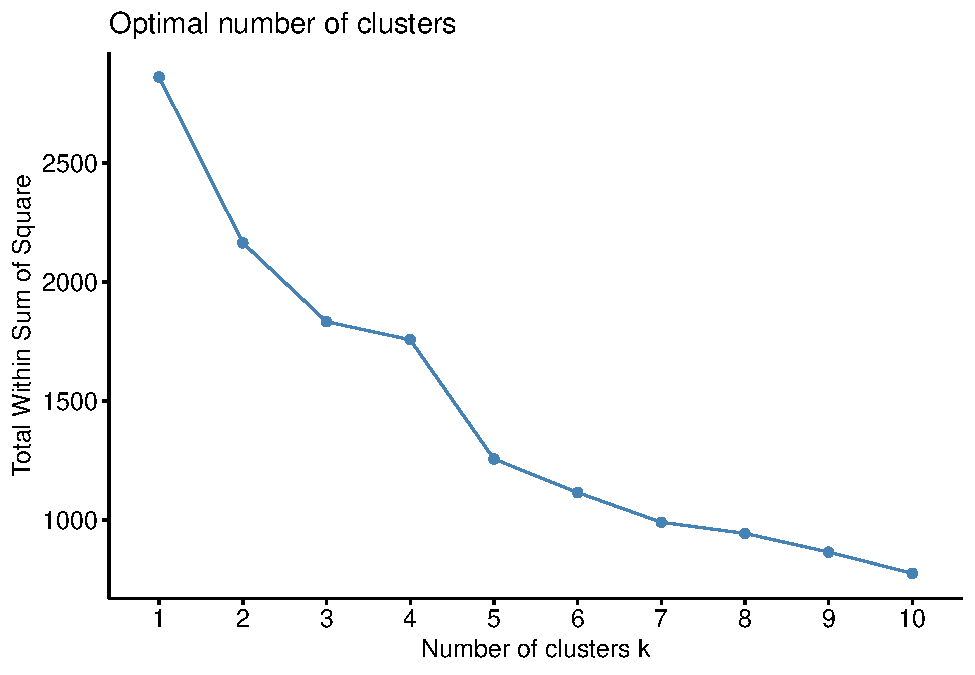
\includegraphics{MSDS680-Week-6-Kmeans-and-HCA_files/figure-latex/kmeans investigation-2.pdf}

\begin{Shaded}
\begin{Highlighting}[]
\KeywordTok{fviz_nbclust}\NormalTok{(clean_customers, kmeans, }\DataTypeTok{method =} \StringTok{'silhouette'}\NormalTok{)}
\end{Highlighting}
\end{Shaded}

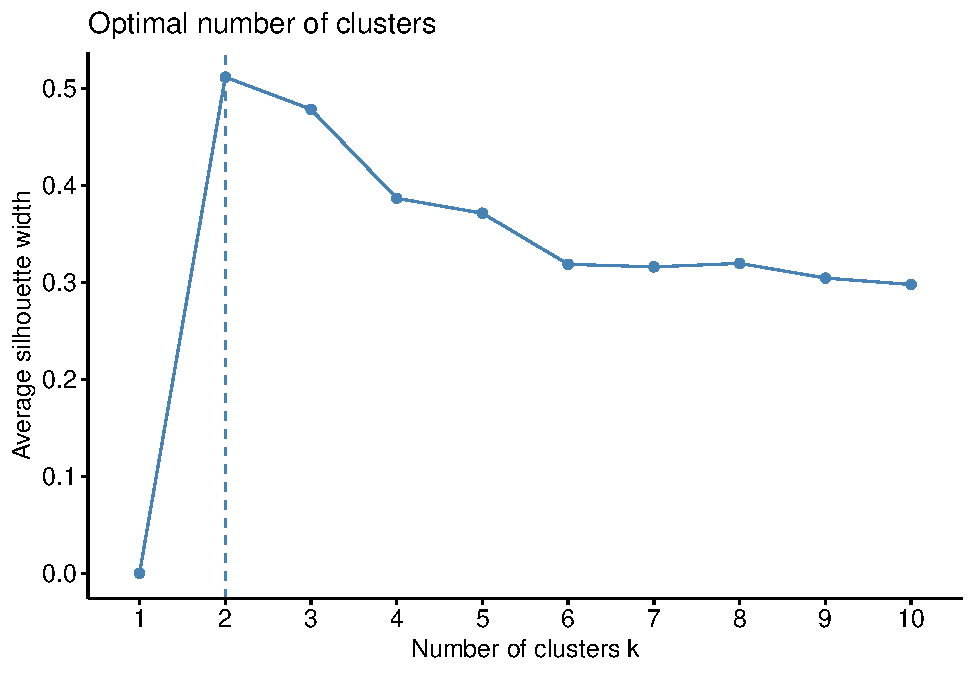
\includegraphics{MSDS680-Week-6-Kmeans-and-HCA_files/figure-latex/kmeans investigation-3.pdf}

\begin{Shaded}
\begin{Highlighting}[]
\KeywordTok{fviz_nbclust}\NormalTok{(scaled_clean_cust, kmeans, }\DataTypeTok{method =} \StringTok{'silhouette'}\NormalTok{)}
\end{Highlighting}
\end{Shaded}

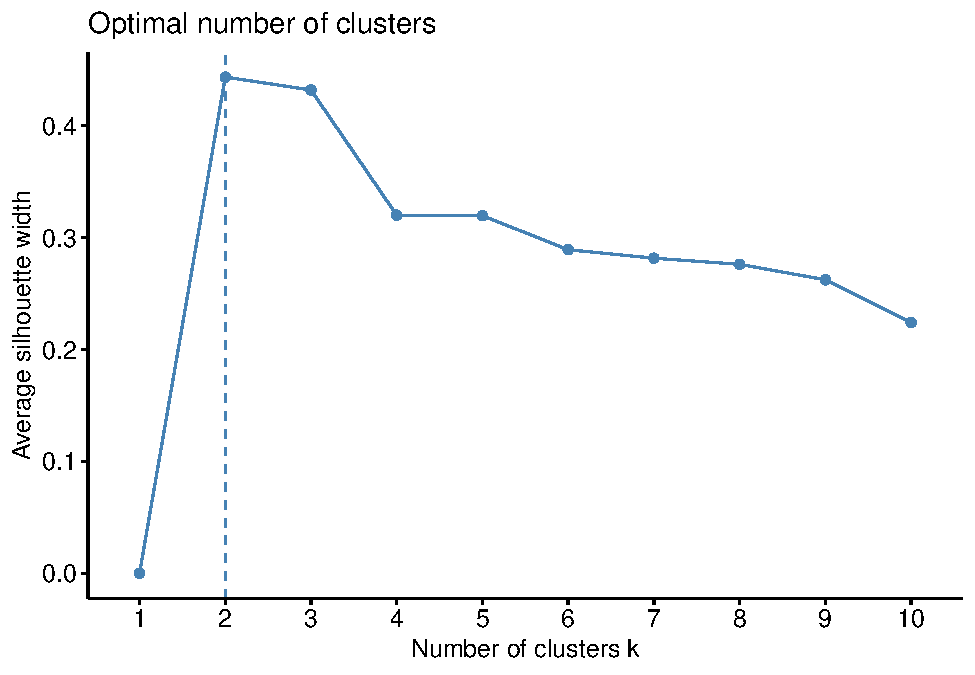
\includegraphics{MSDS680-Week-6-Kmeans-and-HCA_files/figure-latex/kmeans investigation-4.pdf}

\begin{Shaded}
\begin{Highlighting}[]
\KeywordTok{fviz_nbclust}\NormalTok{(clean_customers, kmeans, }\DataTypeTok{method =} \StringTok{'wss'}\NormalTok{) }\OperatorTok{+}
\StringTok{  }\KeywordTok{geom_vline}\NormalTok{(}\DataTypeTok{xintercept =} \DecValTok{5}\NormalTok{, }\DataTypeTok{linetype =} \DecValTok{1}\NormalTok{)}
\end{Highlighting}
\end{Shaded}

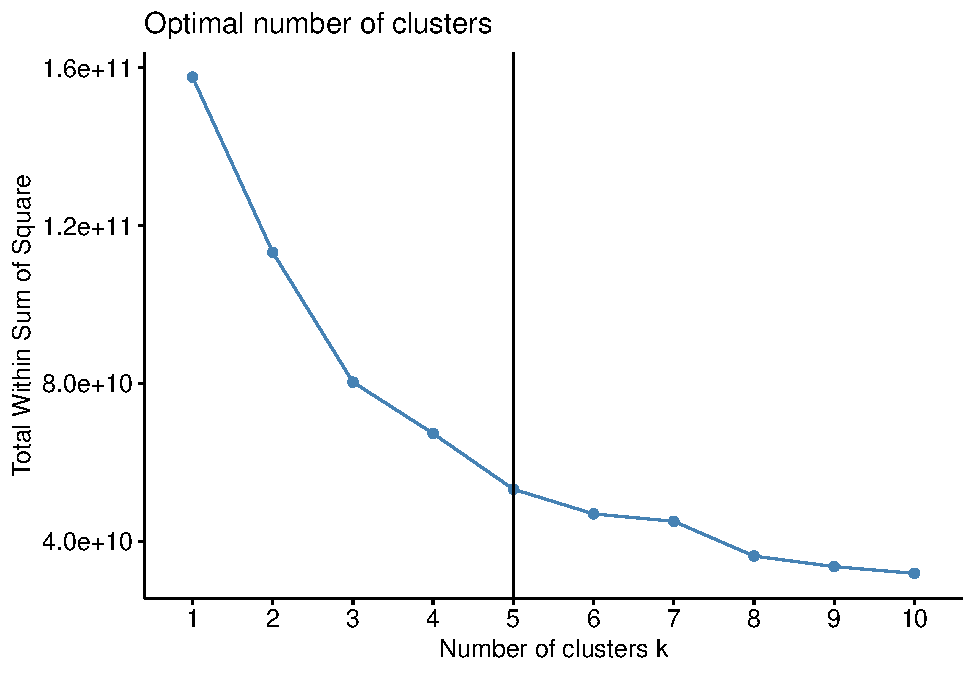
\includegraphics{MSDS680-Week-6-Kmeans-and-HCA_files/figure-latex/kmeans investigation-5.pdf}

\hypertarget{kmeans-model}{%
\subsection{Kmeans Model}\label{kmeans-model}}

\begin{Shaded}
\begin{Highlighting}[]
\NormalTok{kmeans_fit <-}\StringTok{ }\KeywordTok{kmeans}\NormalTok{(clean_customers, }\DecValTok{5}\NormalTok{)}

\NormalTok{kmeans_fit}\OperatorTok{$}\NormalTok{size}
\end{Highlighting}
\end{Shaded}

\begin{verbatim}
## [1] 113  24 227   5  71
\end{verbatim}

\begin{Shaded}
\begin{Highlighting}[]
\NormalTok{kmeans_fit}\OperatorTok{$}\NormalTok{centers}
\end{Highlighting}
\end{Shaded}

\begin{verbatim}
##    Channel.2   Region.2  Region.3     Fresh      Milk   Grocery   Frozen
## 1 0.19469027 0.11504425 0.7168142 20600.283  3787.832  5089.841 3989.071
## 2 0.08333333 0.04166667 0.8333333 48777.375  6607.375  6197.792 9462.792
## 3 0.20264317 0.09691630 0.7224670  5655.819  3567.793  4513.040 2386.529
## 4 1.00000000 0.20000000 0.8000000 25603.000 43460.600 61472.200 2636.000
## 5 0.94366197 0.14084507 0.6619718  5207.831 13191.028 20321.718 1674.028
##   Detergents_Paper Delicassen
## 1         1130.142   1639.071
## 2          932.125   4435.333
## 3         1437.559   1005.031
## 4        29974.200   2708.800
## 5         9036.380   1937.944
\end{verbatim}

\begin{Shaded}
\begin{Highlighting}[]
\NormalTok{(kmeans_fit}\OperatorTok{$}\NormalTok{betweenss}\OperatorTok{/}\NormalTok{kmeans_fit}\OperatorTok{$}\NormalTok{totss) }\CommentTok{#provides fit score}
\end{Highlighting}
\end{Shaded}

\begin{verbatim}
## [1] 0.6629548
\end{verbatim}

\hypertarget{feature-compare}{%
\subsection{Feature Compare}\label{feature-compare}}

\begin{Shaded}
\begin{Highlighting}[]
\CommentTok{#gives all the plots to provide a good candidate for inspection}
\KeywordTok{plot}\NormalTok{(clean_customers, }\DataTypeTok{col=}\NormalTok{kmeans_fit}\OperatorTok{$}\NormalTok{cluster) }
\end{Highlighting}
\end{Shaded}

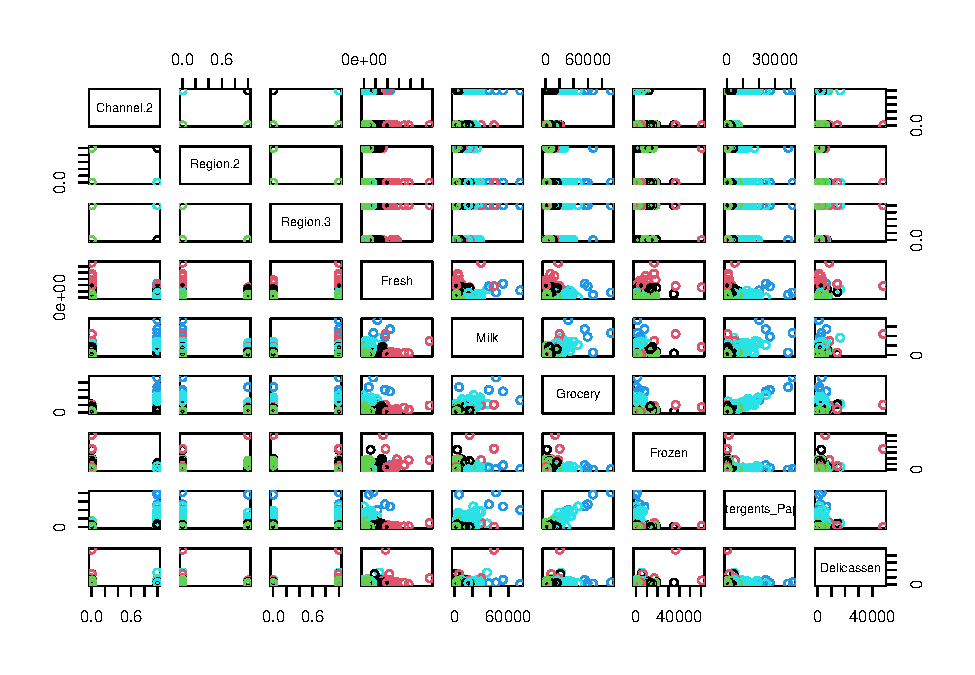
\includegraphics{MSDS680-Week-6-Kmeans-and-HCA_files/figure-latex/kmeans plots-1.pdf}

\begin{Shaded}
\begin{Highlighting}[]
\KeywordTok{plot}\NormalTok{(clean_customers[}\KeywordTok{c}\NormalTok{(}\StringTok{'Fresh'}\NormalTok{,}\StringTok{'Detergents_Paper'}\NormalTok{)], }\DataTypeTok{col=}\NormalTok{kmeans_fit}\OperatorTok{$}\NormalTok{cluster)}
\CommentTok{#adds center of cluster to plot}
\KeywordTok{points}\NormalTok{(kmeans_fit}\OperatorTok{$}\NormalTok{centers[,}\KeywordTok{c}\NormalTok{(}\StringTok{'Fresh'}\NormalTok{, }\StringTok{'Detergents_Paper'}\NormalTok{)], }
       \DataTypeTok{col=}\DecValTok{1}\OperatorTok{:}\DecValTok{5}\NormalTok{, }\DataTypeTok{pch=}\DecValTok{8}\NormalTok{, }\DataTypeTok{cex=}\DecValTok{2}\NormalTok{) }
\end{Highlighting}
\end{Shaded}

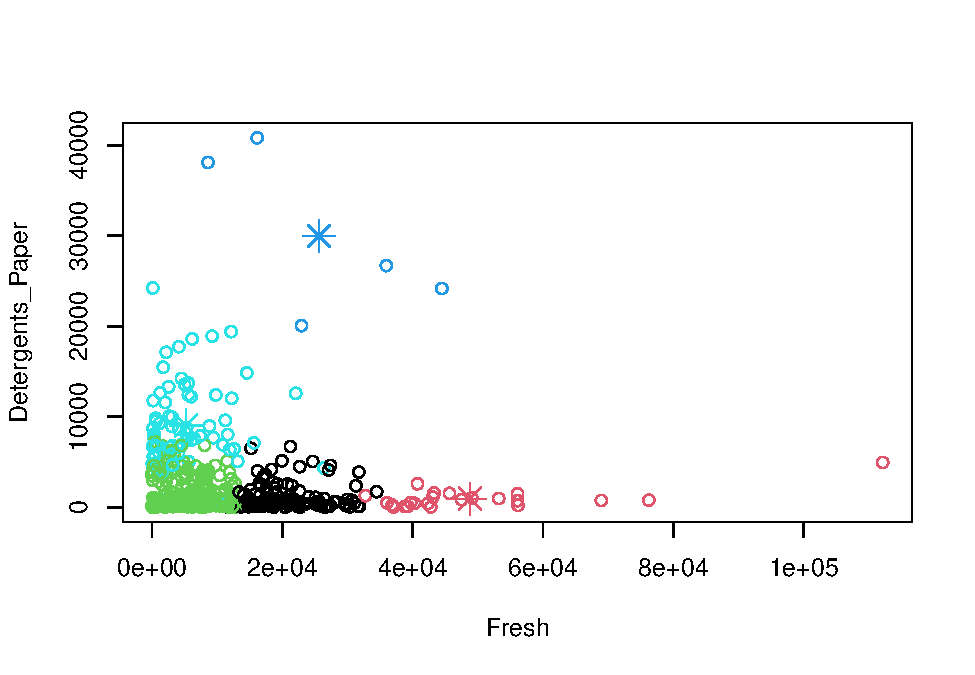
\includegraphics{MSDS680-Week-6-Kmeans-and-HCA_files/figure-latex/kmeans plots-2.pdf}

\hypertarget{kmeans-analysis}{%
\subsection{Kmeans analysis}\label{kmeans-analysis}}

\begin{Shaded}
\begin{Highlighting}[]
\NormalTok{clean_customers}\OperatorTok{$}\NormalTok{kmeans_cluster <-}\StringTok{ }\NormalTok{kmeans_fit}\OperatorTok{$}\NormalTok{cluster}

\KeywordTok{head}\NormalTok{(clean_customers)}
\end{Highlighting}
\end{Shaded}

\begin{verbatim}
##   Channel.2 Region.2 Region.3 Fresh Milk Grocery Frozen Detergents_Paper
## 1         1        0        1 12669 9656    7561    214             2674
## 2         1        0        1  7057 9810    9568   1762             3293
## 3         1        0        1  6353 8808    7684   2405             3516
## 4         0        0        1 13265 1196    4221   6404              507
## 5         1        0        1 22615 5410    7198   3915             1777
## 6         1        0        1  9413 8259    5126    666             1795
##   Delicassen kmeans_cluster
## 1       1338              3
## 2       1776              3
## 3       7844              3
## 4       1788              1
## 5       5185              1
## 6       1451              3
\end{verbatim}

\begin{Shaded}
\begin{Highlighting}[]
\CommentTok{# summary statistics grouped by cluster}
\KeywordTok{aggregate}\NormalTok{(clean_customers, }\KeywordTok{list}\NormalTok{(clean_customers}\OperatorTok{$}\NormalTok{kmeans_cluster), min) }
\end{Highlighting}
\end{Shaded}

\begin{verbatim}
##   Group.1 Channel.2 Region.2 Region.3 Fresh Milk Grocery Frozen
## 1       1         0        0        0 11314  134       3    118
## 2       2         0        0        0 32717  286     471    532
## 3       3         0        0        0     3   55     137     25
## 4       4         1        0        0  8565 4980   32114    131
## 5       5         0        0        0    18 1275   10487     33
##   Detergents_Paper Delicassen kmeans_cluster
## 1                3         57              1
## 2               20          3              2
## 3                3          3              3
## 4            20070        903              4
## 5              282          3              5
\end{verbatim}

\begin{Shaded}
\begin{Highlighting}[]
\KeywordTok{aggregate}\NormalTok{(clean_customers, }\KeywordTok{list}\NormalTok{(clean_customers}\OperatorTok{$}\NormalTok{kmeans_cluster), max)}
\end{Highlighting}
\end{Shaded}

\begin{verbatim}
##   Group.1 Channel.2 Region.2 Region.3  Fresh  Milk Grocery Frozen
## 1       1         1        1        1  34454 16687   21042  35009
## 2       2         1        1        1 112151 43950   20170  60869
## 3       3         1        1        1  13146 18664   16483  17866
## 4       4         1        1        1  44466 73498   92780   7782
## 5       5         1        1        1  26373 36423   45828  10155
##   Detergents_Paper Delicassen kmeans_cluster
## 1             6707      14472              1
## 2             4948      47943              2
## 3             7271       7844              3
## 4            40827       6465              4
## 5            24231      16523              5
\end{verbatim}

\begin{Shaded}
\begin{Highlighting}[]
\KeywordTok{aggregate}\NormalTok{(clean_customers, }\KeywordTok{list}\NormalTok{(clean_customers}\OperatorTok{$}\NormalTok{kmeans_cluster), mean)}
\end{Highlighting}
\end{Shaded}

\begin{verbatim}
##   Group.1  Channel.2   Region.2  Region.3     Fresh      Milk   Grocery
## 1       1 0.19469027 0.11504425 0.7168142 20600.283  3787.832  5089.841
## 2       2 0.08333333 0.04166667 0.8333333 48777.375  6607.375  6197.792
## 3       3 0.20264317 0.09691630 0.7224670  5655.819  3567.793  4513.040
## 4       4 1.00000000 0.20000000 0.8000000 25603.000 43460.600 61472.200
## 5       5 0.94366197 0.14084507 0.6619718  5207.831 13191.028 20321.718
##     Frozen Detergents_Paper Delicassen kmeans_cluster
## 1 3989.071         1130.142   1639.071              1
## 2 9462.792          932.125   4435.333              2
## 3 2386.529         1437.559   1005.031              3
## 4 2636.000        29974.200   2708.800              4
## 5 1674.028         9036.380   1937.944              5
\end{verbatim}

\hypertarget{hca-cluster-decision}{%
\subsection{HCA Cluster Decision}\label{hca-cluster-decision}}

\begin{Shaded}
\begin{Highlighting}[]
\KeywordTok{fviz_nbclust}\NormalTok{(clean_customers, hcut, }\DataTypeTok{method  =} \StringTok{'wss'}\NormalTok{) }\CommentTok{#hca plot with wss}
\end{Highlighting}
\end{Shaded}

\includegraphics{MSDS680-Week-6-Kmeans-and-HCA_files/figure-latex/hca vis \& dist-1.pdf}

\begin{Shaded}
\begin{Highlighting}[]
\KeywordTok{fviz_nbclust}\NormalTok{(clean_customers, hcut, }\DataTypeTok{method  =} \StringTok{'silhouette'}\NormalTok{) }\CommentTok{#hca silhouette}
\end{Highlighting}
\end{Shaded}

\includegraphics{MSDS680-Week-6-Kmeans-and-HCA_files/figure-latex/hca vis \& dist-2.pdf}

\begin{Shaded}
\begin{Highlighting}[]
\CommentTok{#agglomerative distance between points using euclidean }
\NormalTok{agg_d <-}\StringTok{ }\KeywordTok{dist}\NormalTok{(clean_customers, }\DataTypeTok{method =} \StringTok{'euclidean'}\NormalTok{) }
\end{Highlighting}
\end{Shaded}

\hypertarget{agglomerative}{%
\subsection{Agglomerative}\label{agglomerative}}

\hypertarget{complete}{%
\subsubsection{Complete}\label{complete}}

\begin{Shaded}
\begin{Highlighting}[]
\NormalTok{hc_complete_agg <-}\StringTok{ }\KeywordTok{hclust}\NormalTok{(agg_d, }\DataTypeTok{method =} \StringTok{'complete'}\NormalTok{) }\CommentTok{#HCA using complete method}
\KeywordTok{plot}\NormalTok{(hc_complete_agg, }\DataTypeTok{cex =}\NormalTok{.}\DecValTok{6}\NormalTok{, }\DataTypeTok{hang =} \DecValTok{-1}\NormalTok{)}
\end{Highlighting}
\end{Shaded}

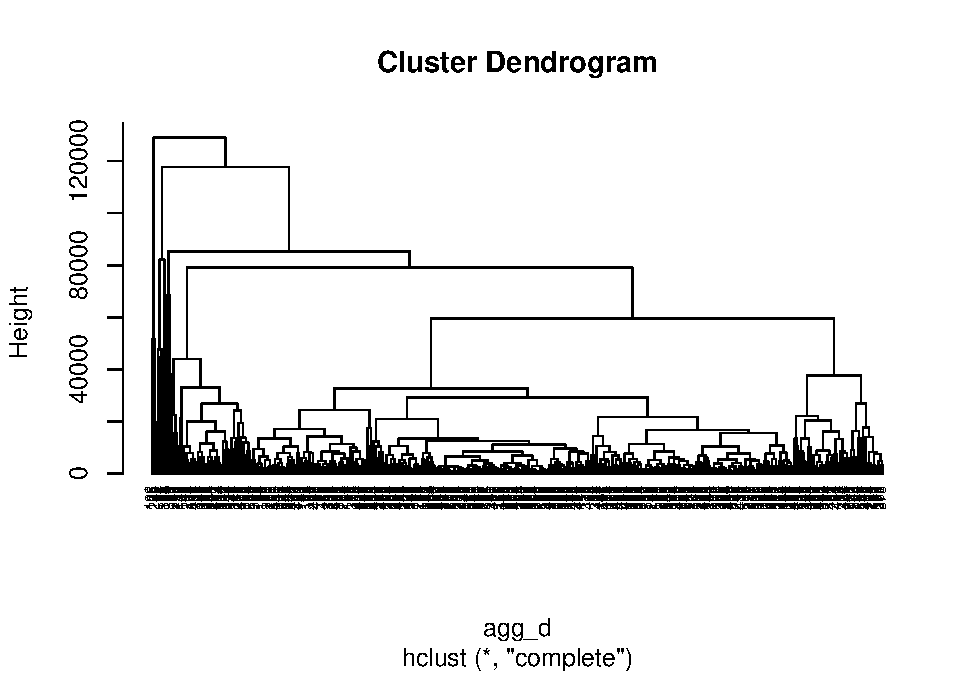
\includegraphics{MSDS680-Week-6-Kmeans-and-HCA_files/figure-latex/complete-1.pdf}

\begin{Shaded}
\begin{Highlighting}[]
\NormalTok{hc_complete_agg_fit <-}\StringTok{ }\KeywordTok{cutree}\NormalTok{(hc_complete_agg, }\DataTypeTok{k=}\DecValTok{3}\NormalTok{) }\CommentTok{#splits HCA into 3 clusters}

\KeywordTok{table}\NormalTok{(hc_complete_agg_fit) }\CommentTok{#number of data points in each cluster}
\end{Highlighting}
\end{Shaded}

\begin{verbatim}
## hc_complete_agg_fit
##   1   2   3 
## 431   6   3
\end{verbatim}

\begin{Shaded}
\begin{Highlighting}[]
\KeywordTok{plot}\NormalTok{(hc_complete_agg)}
\KeywordTok{rect.hclust}\NormalTok{(hc_complete_agg, }\DataTypeTok{k=}\DecValTok{3}\NormalTok{) }\CommentTok{#addes cluster split}
\end{Highlighting}
\end{Shaded}

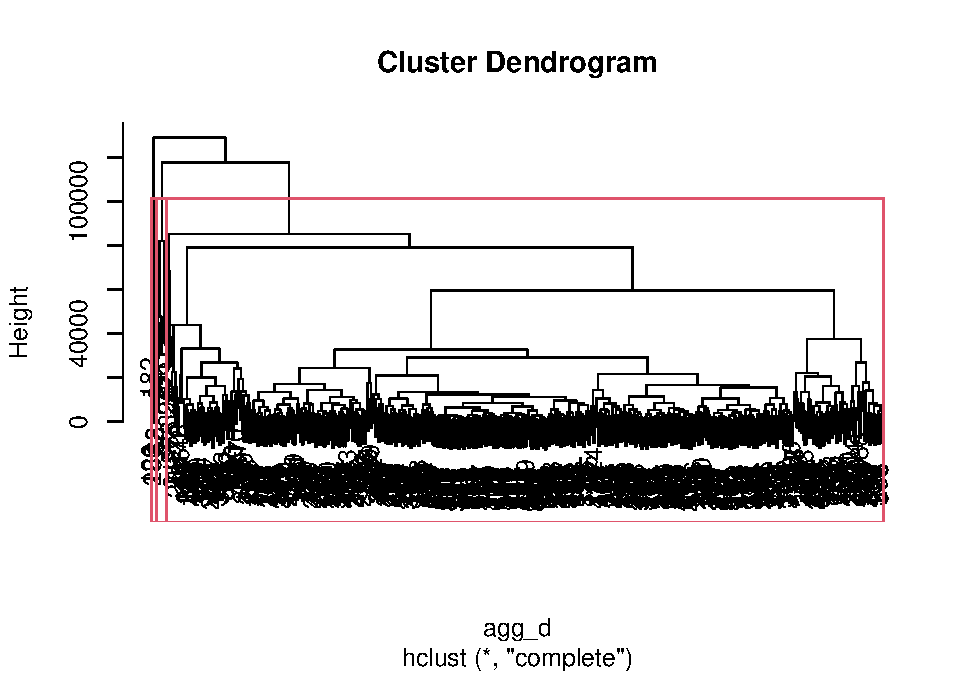
\includegraphics{MSDS680-Week-6-Kmeans-and-HCA_files/figure-latex/complete-2.pdf}

\hypertarget{ward-1}{%
\subsubsection{Ward-1}\label{ward-1}}

\begin{Shaded}
\begin{Highlighting}[]
\NormalTok{hc_wd2 <-}\StringTok{ }\KeywordTok{hclust}\NormalTok{(agg_d, }\DataTypeTok{method =} \StringTok{'ward.D2'}\NormalTok{)}
\KeywordTok{plot}\NormalTok{(hc_wd2, }\DataTypeTok{cex =}\NormalTok{.}\DecValTok{6}\NormalTok{, }\DataTypeTok{hang =} \DecValTok{-1}\NormalTok{)}
\end{Highlighting}
\end{Shaded}

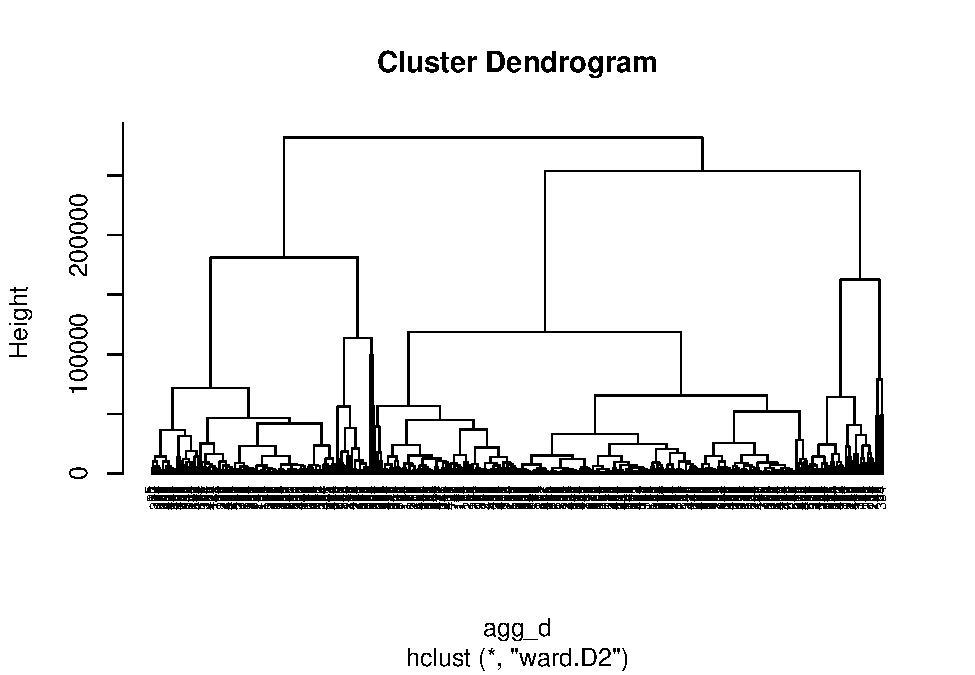
\includegraphics{MSDS680-Week-6-Kmeans-and-HCA_files/figure-latex/ward2-1.pdf}

\begin{Shaded}
\begin{Highlighting}[]
\NormalTok{hc_wd2_fit <-}\StringTok{ }\KeywordTok{cutree}\NormalTok{(hc_wd2, }\DataTypeTok{k =} \DecValTok{3}\NormalTok{)}

\KeywordTok{table}\NormalTok{(hc_wd2_fit)}
\end{Highlighting}
\end{Shaded}

\begin{verbatim}
## hc_wd2_fit
##   1   2   3 
## 261 134  45
\end{verbatim}

\begin{Shaded}
\begin{Highlighting}[]
\KeywordTok{plot}\NormalTok{(hc_wd2)}
\KeywordTok{rect.hclust}\NormalTok{(hc_wd2, }\DataTypeTok{k =} \DecValTok{3}\NormalTok{, }\DataTypeTok{border =} \DecValTok{2}\OperatorTok{:}\DecValTok{5}\NormalTok{)}
\end{Highlighting}
\end{Shaded}

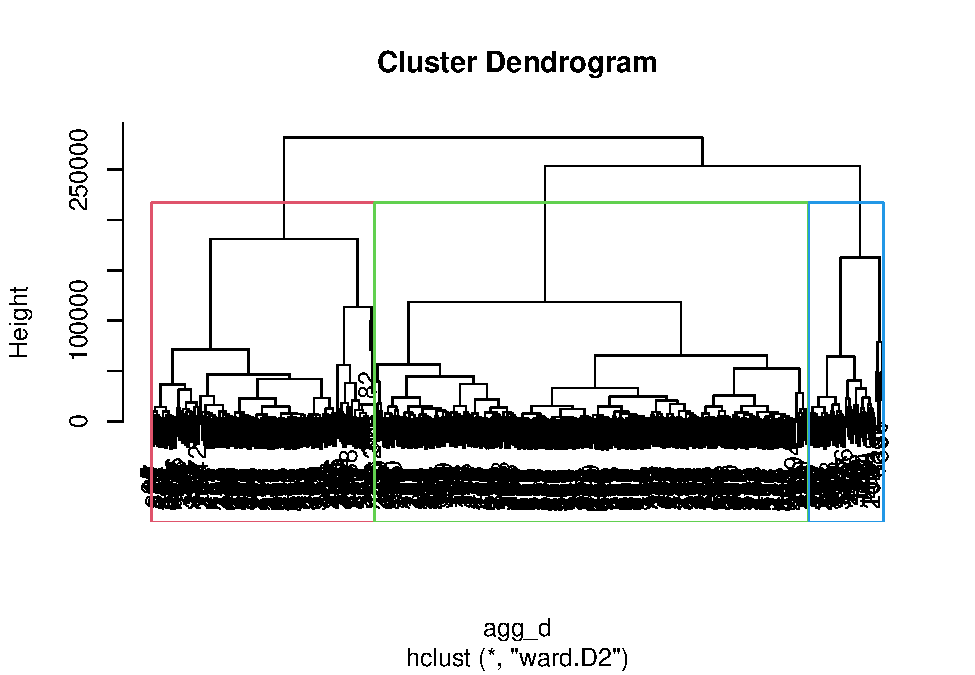
\includegraphics{MSDS680-Week-6-Kmeans-and-HCA_files/figure-latex/ward2-2.pdf}

\hypertarget{ward-2}{%
\subsubsection{Ward-2}\label{ward-2}}

\begin{Shaded}
\begin{Highlighting}[]
\NormalTok{hc_wd2_new_fit <-}\StringTok{ }\KeywordTok{cutree}\NormalTok{(hc_wd2, }\DataTypeTok{h =} \DecValTok{175000}\NormalTok{) }\CommentTok{#splits hca based off height}

\KeywordTok{table}\NormalTok{(hc_wd2_new_fit)}
\end{Highlighting}
\end{Shaded}

\begin{verbatim}
## hc_wd2_new_fit
##   1   2   3   4 
## 261 111  45  23
\end{verbatim}

\begin{Shaded}
\begin{Highlighting}[]
\KeywordTok{plot}\NormalTok{(hc_wd2)}
\KeywordTok{rect.hclust}\NormalTok{(hc_wd2, }\DataTypeTok{h =} \DecValTok{175000}\NormalTok{, }\DataTypeTok{border =} \DecValTok{2}\OperatorTok{:}\DecValTok{5}\NormalTok{)}
\end{Highlighting}
\end{Shaded}

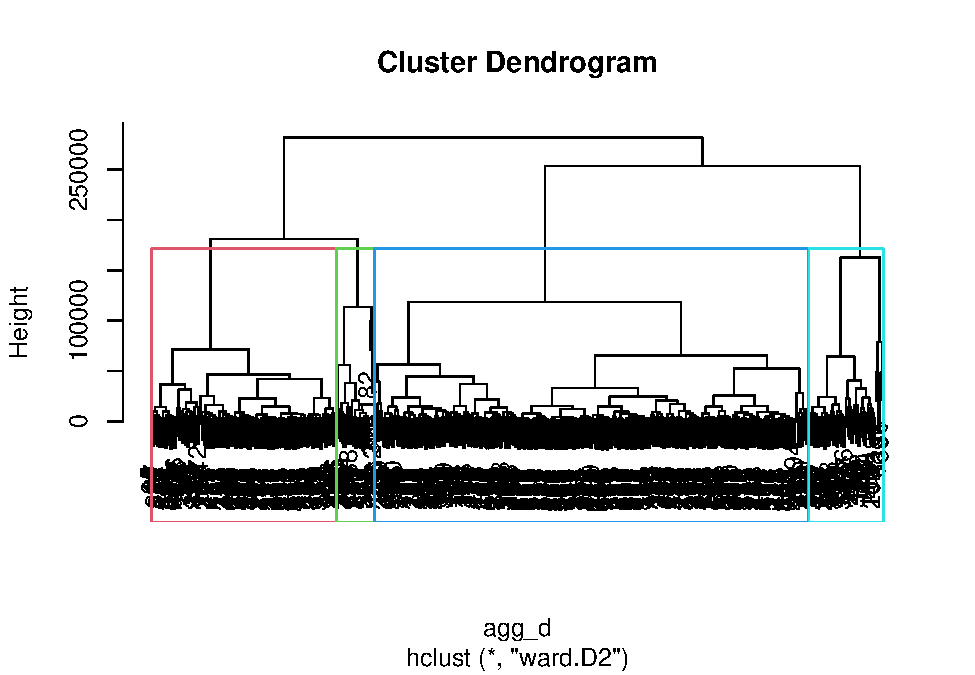
\includegraphics{MSDS680-Week-6-Kmeans-and-HCA_files/figure-latex/ward2 new height-1.pdf}

\begin{Shaded}
\begin{Highlighting}[]
\KeywordTok{fviz_cluster}\NormalTok{(}\KeywordTok{list}\NormalTok{(}\DataTypeTok{data =}\NormalTok{ clean_customers[,}\KeywordTok{c}\NormalTok{(}\DecValTok{1}\OperatorTok{:}\DecValTok{9}\NormalTok{)], }
                  \DataTypeTok{cluster =}\NormalTok{ hc_wd2_new_fit)) }\CommentTok{#provides cluster plot of clusters}
\end{Highlighting}
\end{Shaded}

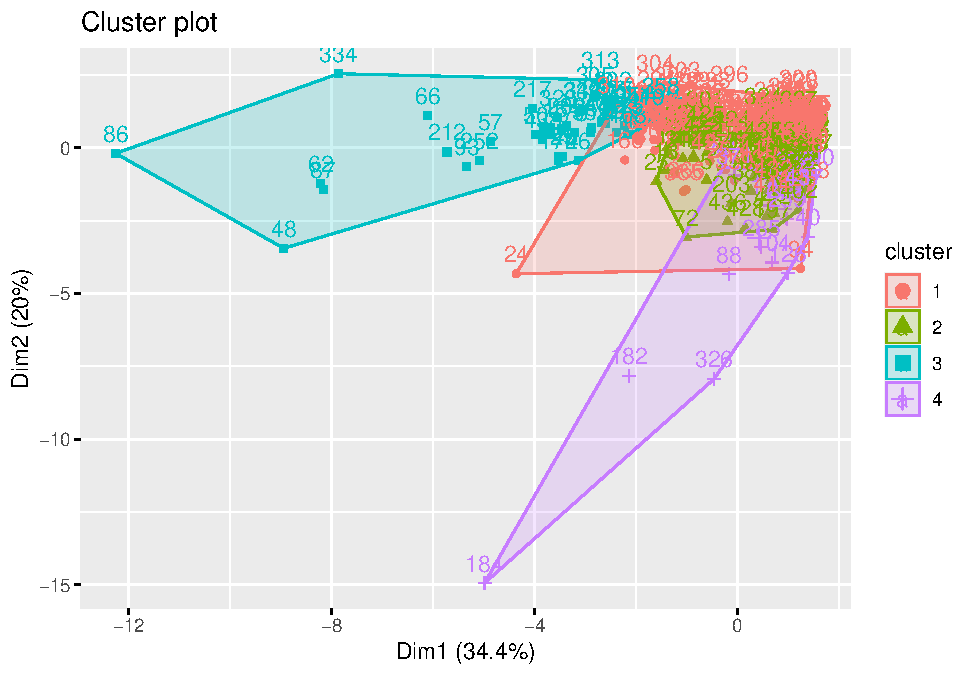
\includegraphics{MSDS680-Week-6-Kmeans-and-HCA_files/figure-latex/ward2 new height-2.pdf}

\hypertarget{divisive}{%
\subsection{Divisive}\label{divisive}}

\begin{Shaded}
\begin{Highlighting}[]
\NormalTok{div_d <-}\StringTok{ }\KeywordTok{diana}\NormalTok{(clean_customers, }\DataTypeTok{metric =} \StringTok{'euclidean'}\NormalTok{) }\CommentTok{#divisive hca}

\KeywordTok{plot}\NormalTok{(div_d, }\DataTypeTok{which.plots =} \DecValTok{2}\NormalTok{)}
\end{Highlighting}
\end{Shaded}

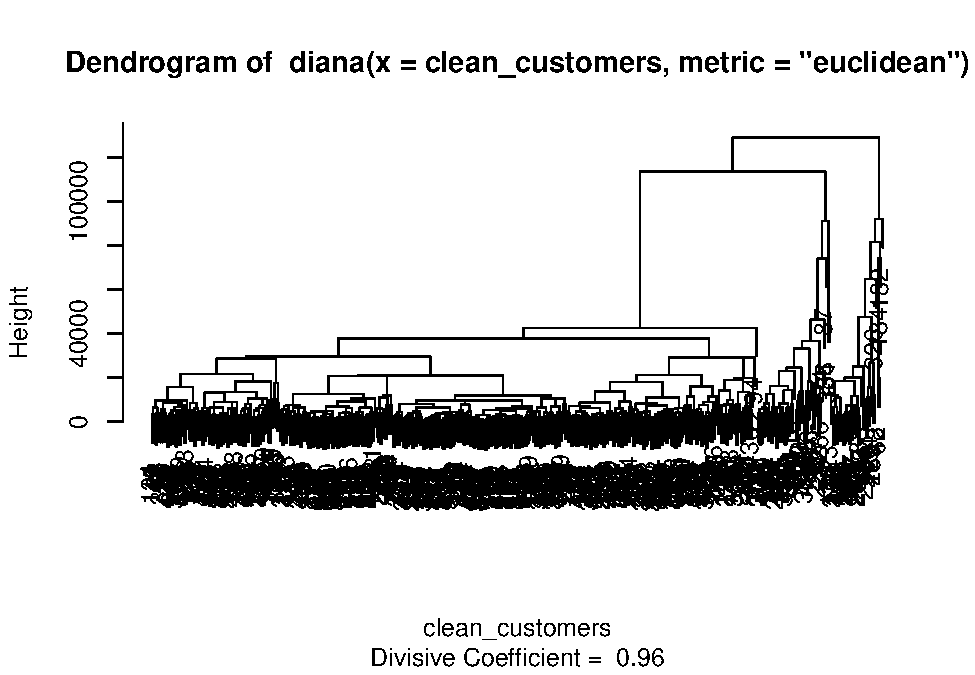
\includegraphics{MSDS680-Week-6-Kmeans-and-HCA_files/figure-latex/divisive-1.pdf}

\begin{Shaded}
\begin{Highlighting}[]
\NormalTok{div_cut <-}\StringTok{ }\KeywordTok{cutree}\NormalTok{(div_d, }\DataTypeTok{k=}\DecValTok{3}\NormalTok{)}
\KeywordTok{table}\NormalTok{(div_cut)}
\end{Highlighting}
\end{Shaded}

\begin{verbatim}
## div_cut
##   1   2   3 
## 364  44  32
\end{verbatim}

\begin{Shaded}
\begin{Highlighting}[]
\NormalTok{div_d}\OperatorTok{$}\NormalTok{dc}
\end{Highlighting}
\end{Shaded}

\begin{verbatim}
## [1] 0.9633628
\end{verbatim}

\begin{Shaded}
\begin{Highlighting}[]
\KeywordTok{fviz_cluster}\NormalTok{(}\KeywordTok{list}\NormalTok{(}\DataTypeTok{data =}\NormalTok{ clean_customers[,}\KeywordTok{c}\NormalTok{(}\DecValTok{1}\OperatorTok{:}\DecValTok{9}\NormalTok{)], }\DataTypeTok{cluster =}\NormalTok{ div_cut))}
\end{Highlighting}
\end{Shaded}

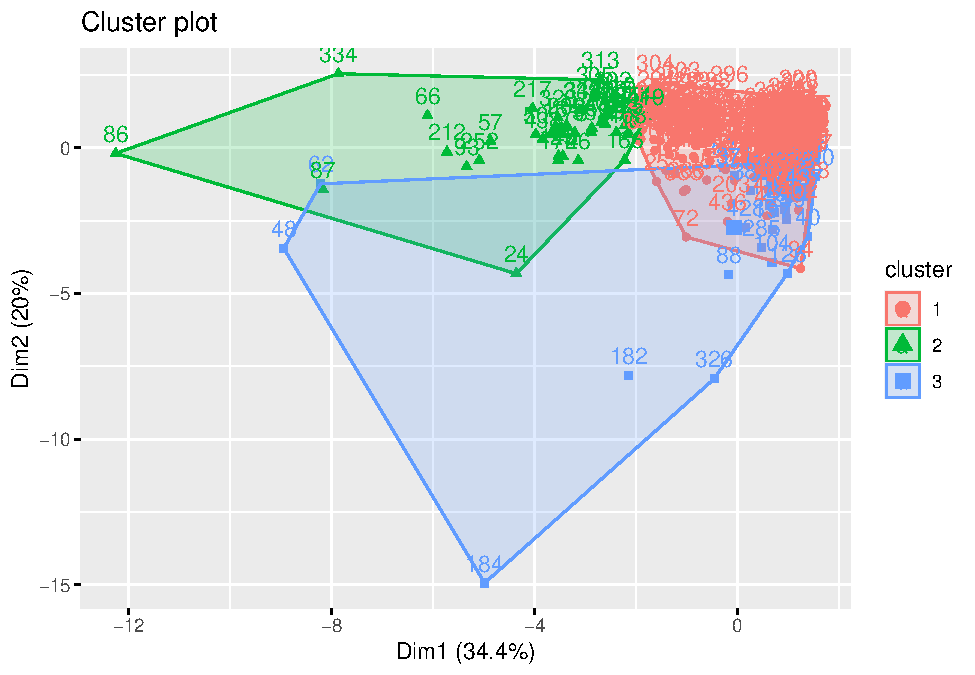
\includegraphics{MSDS680-Week-6-Kmeans-and-HCA_files/figure-latex/divisive-2.pdf}

\hypertarget{hca-analysis}{%
\subsection{HCA Analysis}\label{hca-analysis}}

\hypertarget{conclusion}{%
\section{Conclusion}\label{conclusion}}

\newpage

\hypertarget{references}{%
\section{References}\label{references}}

\begingroup
\setlength{\parindent}{-0.5in}
\setlength{\leftskip}{0.5in}

\hypertarget{refs}{}

\endgroup


\end{document}
